\begin{maintask}{4-2}
  \subsection*{課題内容}
  \texttt{socket\_dns\_test.py}がDNS問い合わせに設定した乱数のQuery IDと，応答パケットのResponse IDが一致することを確認する．

  \subsection*{実験方法}
  \begin{enumerate}
    \item DNS問い合わせのパケットをキャプチャする．
      \begin{minted}{zsh}
        cd ~/socket
        tcpdump -i eth1 -s 0 -w day4_2_dns.pcap 'not port 4200'
      \end{minted}
    \item 別の端末でプログラムを実行する．引数には実際に問い合わせたホスト名を指定する．
      \begin{minted}{zsh}
        cd ~/socket
        ./socket_dns_test.py www.iic.hokudai.ac.jp
      \end{minted}
    \item キャプチャを停止し，pcapをWiresharkで開いてDNSのQueryとResponseを確認する．
  \end{enumerate}

  \subsection*{結果}
  プログラムの実行結果を出力\ref{out:dns_test}に示す．Wiresharkで確認したQuery IDとResponse IDを図\ref{fig:dns_id}に示す．
  使用した\texttt{socket\_dns\_test.py}のソースコードをリスト\ref{lst:dns_test_source}に示す．
  \begin{listing}[H]
    \caption{socket\_dns\_test.py のソースコード（1/4）}\label{lst:dns_test_source}
    \inputminted[fontsize=\scriptsize,firstline=1,lastline=33]{python}{src/day4/socket_dns_test.py}
  \end{listing}
  \begin{listing}[H]
    \caption{socket\_dns\_test.py のソースコード（2/4）}
    \inputminted[fontsize=\scriptsize,firstline=34,lastline=66]{python}{src/day4/socket_dns_test.py}
  \end{listing}
  \begin{listing}[H]
    \caption{socket\_dns\_test.py のソースコード（3/4）}
    \inputminted[fontsize=\scriptsize,firstline=67,lastline=99]{python}{src/day4/socket_dns_test.py}
  \end{listing}
  \begin{listing}[H]
    \caption{socket\_dns\_test.py のソースコード（4/4）}
    \inputminted[fontsize=\scriptsize,firstline=100,lastline=132]{python}{src/day4/socket_dns_test.py}
  \end{listing}

  \begin{termout}[H]
    \caption{socket\_dns\_test.py の実行結果}\label{out:dns_test}
    \begin{minted}{text}
    guest@host82:~/socket$ ./socket_dns_test.py www.iic.hokudai.ac.jp
    id = 52921                                                                                                    
    [(b'www.iic.hokudai.ac.jp', 1, 1, 86400, '133.50.42.161')]    
    \end{minted}
  \end{termout}
  \begin{figure}[H]
    \centering
    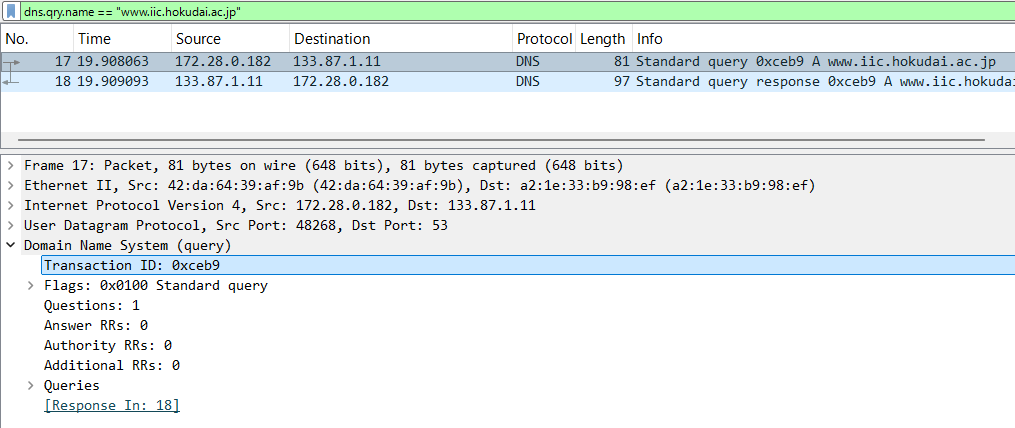
\includegraphics[width=0.98\columnwidth]{fig/wireshark_day4_2_dns_id.png}
    \caption{DNS Query IDとResponse IDの確認}\label{fig:dns_id}
  \end{figure}

  プログラムが表示したIDは10進数で52921，16進数で\texttt{0xceb9}であった．WiresharkでもQueryとResponseのTransaction IDはいずれも\texttt{0xceb9}であり，問い合わせと応答のIDが一致した．
\end{maintask}
